\begin{refsection}

\chapter{Ar--Ar and K--Ca}\label{ch:ArArKCa}

The Ar--Ar and K--Ca chronometers are based on the branched decay of
\textsuperscript{40}K to \textsuperscript{40}Ar and
\textsuperscript{40}Ca. The Ar--Ar is a widely used method that has
replaced the K--Ar method in all but a few applications
(Section~\ref{sec:K-Ar}). The K--Ca method is a more recent
development that has become feasible due to analytical advances in
SIMS, which have resolved the isobaric interference between
\textsuperscript{40}K and \textsuperscript{40}Ca. The original K--Ar
method is not implemented in \texttt{IsoplotR} but may be added later.

\section{Ar--Ar}

\texttt{IsoplotR} offers three input formats for Ar--Ar data, which
all require the user to provide the J factor and its standard error
(Section~\ref{sec:Ar-Ar}), as well as the following columns of
isotopic ratio data:
\begin{enumerate}
\item{`Normal':}
  $\frac{40}{36}$,  
  $\mbox{err}\!\left[\frac{40}{36}\right]$, 
  $\frac{39}{36}$,  
  $\mbox{err}\!\left[\frac{39}{36}\right]$,  
  $\mbox{r}\!\left[\frac{40}{36},\frac{39}{36}\right]$,
  $\left(39\right)$
\item{`Inverse':}
  $\frac{39}{40}$,  
  $\mbox{err}\!\left[\frac{39}{40}\right]$, 
  $\frac{36}{40}$,  
  $\mbox{err}\!\left[\frac{36}{40}\right]$,  
  $\left(\mbox{r}\!\left[\frac{39}{40},\frac{36}{40}\right]\right)$,
  $\left(39\right)$
\item{`Three ratios':}
  $\frac{39}{40}$,  
  $\mbox{err}\!\left[\frac{39}{40}\right]$, 
  $\frac{36}{40}$,  
  $\mbox{err}\!\left[\frac{36}{40}\right]$,  
  $\frac{39}{36}$,  
  $\mbox{err}\!\left[\frac{39}{36}\right]$,
  $\left(39\right)$
\end{enumerate}

\noindent where $(39)$ stands for the amount of \textsuperscript{39}Ar
in each heating step, which is normalised to form the X-axis of an age
spectrum (Section~\ref{sec:agespectra}). Error correlations are much
stronger for format~1 than for format~2 and are therefore compulsory
for the former and optional for the latter. As for the Pb--Pb and
Th--Pb methods, the names of the formats refer to the normal and
inverse isochrons that they form. However, both normal and inverse
isochrons are available for all three methods, because
\texttt{IsoplotR} converts them in the background. It does so using
Equation~\ref{eq:redundantratios} for the conversion from format~3 to
format~2; and using Equation~\ref{eq:format12transformation} to
convert format~2 to format~1 and vice versa.\\

Single grain ages can be calculated by projecting cogenetic aliquots
along an isochron, or by applying a nominal `excess argon' correction
to each aliquot separately. The latter approach typically uses the
atmospheric argon composition, which is characterised by a
\textsuperscript{40}Ar/\textsuperscript{39}Ar ratio of
$298.56\pm{0.31}$ \citet{lee2006}. The resulting ages can then be
visualised as radial plots, KDEs, or CADs:\\

\noindent\begin{minipage}[t][][b]{.7\linewidth}
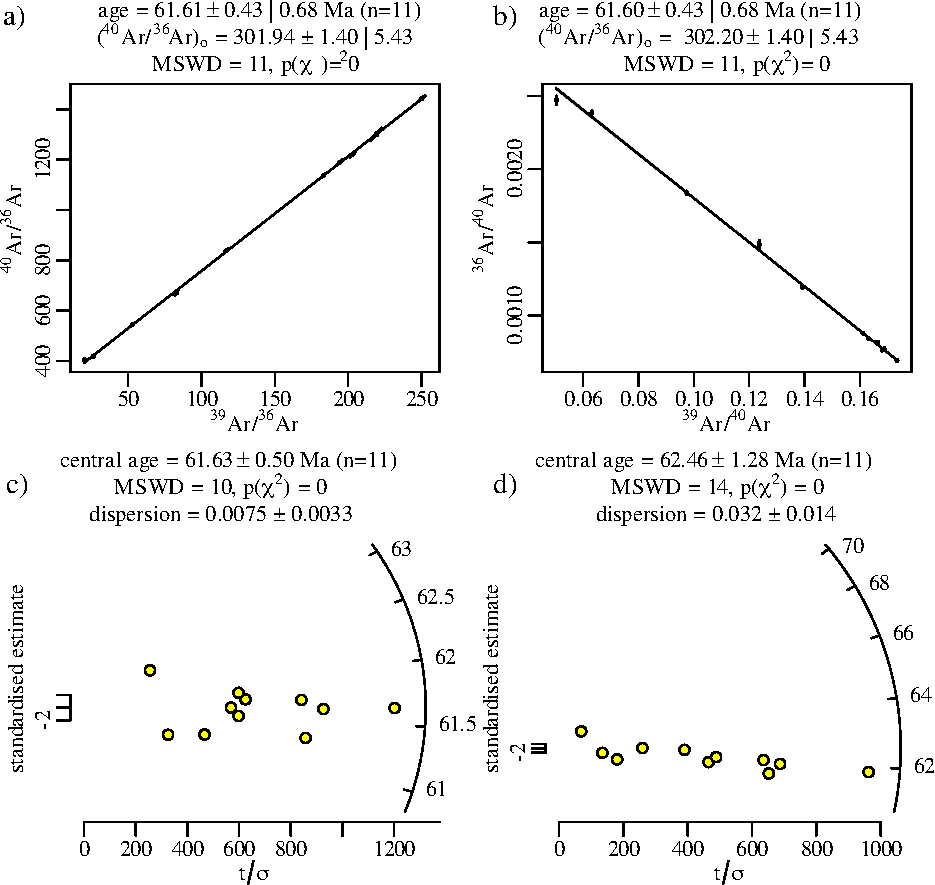
\includegraphics[width=\textwidth]{../figures/ArAr.pdf}
\end{minipage}
\begin{minipage}[t][][t]{.3\linewidth}
  \captionof{figure}{a) conventional and b) inverse model-1 isochron
    for Ar--Ar data. The non-radiogenic (`excess') argon is
    characterised by a \textsuperscript{40}Ar/\textsuperscript{39}Ar
    ratio of 302, which is slightly higher than atmosphere.  c) shows
    a radial plot of the excess-Ar-corrected ages obtained by
    projecting the aliquots along the inverse isochron (just like in
    Figure~\ref{fig:ThPbSingleGrain}.a). d) using the atmospheric
    ratio of $298.56\pm{0.31}$ to correct each aliquot independently
    yields a slightly older and more dispersed distribution.}
  \label{fig:radialArArisochron}
\end{minipage}

\section{Age spectra}\label{sec:agespectra}

As explained in Section~\ref{sec:Ar-Ar}, the
\textsuperscript{40}Ar/\textsuperscript{39}Ar-age spectrum is a useful
tool to visualise stepwise heating measurements. Its appearance is
based on the weighted mean plot (e.g., Figure~\ref{fig:wtdmeanMSWD}),
with the different heating steps arranged in order of increasing
degree of degassing along the horizontal axis, and the width of the
different sample boxes proportional to the corresponding amounts of
\textsuperscript{39}Ar.\\

\texttt{IsoplotR} defines the `plateau age' as the weighted mean age
of the longest sequence (in terms of cumulative \textsuperscript{39}Ar
content) of consecutive heating steps that pass the modified Chauvenet
criterion of Section~\ref{ch:generic}. Note that this definition is
different (and simpler) than the one used by \texttt{Isoplot}
\citep{ludwig2003}. However, it is important to mention that all
definitions of an age plateau are heuristic by nature and should not
be used for quantitative inference.

\begin{center}
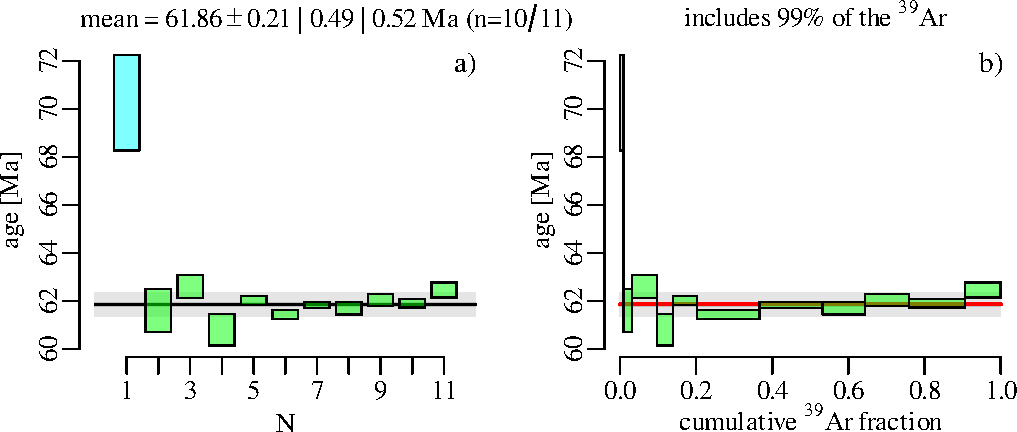
\includegraphics[width=.85\textwidth]{../figures/agespectrum.pdf}
\captionsetup{width=.85\textwidth}
\captionof{figure}{a) weighted mean and b) age spectrum for the Ar--Ar
  of Figure~\ref{fig:radialArArisochron}, using an atmospheric
  \textsuperscript{40}Ar/\textsuperscript{39}Ar-ratio for the
  non-radiogenic component.  The plateau is shown in green and the
  single outlier in blue. The weighted mean age was calculated using
  an ordinary weighted mean. In this case the weighted mean age and
  the plateau age are the same but this is not always the case.}
\label{fig:agespectrum}
\end{center}

\section{K--Ca}\label{sec:K-Ca}

\texttt{IsoplotR} offers three input formats for K--Ca data:
\begin{enumerate}
\item{`Normal':}
  $\frac{{}^{40}\mbox{K}}{{}^{44}\mbox{Ca}}$,  
  $\mbox{err}\!\left[\frac{{}^{40}\mbox{Ca}}{{}^{44}\mbox{Ca}}\right]$, 
  $\frac{{}^{40}\mbox{Ca}}{{}^{44}\mbox{Ca}}$,
  $\mbox{err}\!\left[\frac{{}^{40}\mbox{Ca}}{{}^{44}\mbox{Ca}}\right]$,  
  $\mbox{r}\!\left[\frac{{}^{40}\mbox{K}}{{}^{44}\mbox{Ca}},
    \frac{{}^{40}\mbox{Ca}}{{}^{44}\mbox{Ca}}\right]$
\item{`Inverse':}
  $\frac{{}^{40}\mbox{K}}{{}^{40}\mbox{Ca}}$,  
  $\mbox{err}\!\left[\frac{{}^{40}\mbox{K}}{{}^{40}\mbox{Ca}}\right]$, 
  $\frac{{}^{44}\mbox{Ca}}{{}^{40}\mbox{Ca}}$,  
  $\mbox{err}\!\left[\frac{{}^{40}\mbox{Ca}}{{}^{40}\mbox{Ca}}\right]$,  
  $\mbox{r}\!\left[\frac{{}^{40}\mbox{K}}{{}^{40}\mbox{Ca}},
    \frac{{}^{44}\mbox{Ca}}{{}^{40}\mbox{Ca}}\right]$
\item{`Three ratios':}
  $\frac{{}^{40}\mbox{K}}{{}^{40}\mbox{Ca}}$,  
  $\mbox{err}\!\left[\frac{{}^{40}\mbox{K}}{{}^{40}\mbox{Ca}}\right]$, 
  $\frac{{}^{44}\mbox{Ca}}{{}^{40}\mbox{Ca}}$,  
  $\mbox{err}\!\left[\frac{{}^{40}\mbox{Ca}}{{}^{40}\mbox{Ca}}\right]$,  
  $\mbox{r}\!\left[\frac{{}^{40}\mbox{K}}{{}^{40}\mbox{Ca}},
    \frac{{}^{44}\mbox{Ca}}{{}^{40}\mbox{Ca}}\right]$,
  $\frac{{}^{40}\mbox{K}}{{}^{40}\mbox{Ca}}$,  
  $\mbox{err}\!\left[\frac{{}^{40}\mbox{K}}{{}^{40}\mbox{Ca}}\right]$
\end{enumerate}

\noindent where, in contrast with previous formatting summaries, the
full names of the nuclides are given because of the isobaric parent
and daughter. It is precisely this isobary that prevented the K--Ca
from being widely applied until recently. Formats~1, 2 and 3 can be
converted to each other using Equations~\ref{eq:redundantratios} and
\ref{eq:format12transformation}.\\

\texttt{IsoplotR} uses \textsuperscript{44}Ca as a normalising isotope
because it is the most abundant of calcium's non-radiogenic isotopes,
accounting for up to 2\% of the isotopic budget. Using a less abundant
isotope such as \textsuperscript{42}Ca ($<0.647\%$),
\textsuperscript{43}Ca ($<0.135\%$), or \textsuperscript{46}Ca
($<0.004\%$), would only increase the error correlations in
conventional isochron space (which are already very strong as shown in
Figure~\ref{fig:errorcorrelation}). However, \texttt{IsoplotR} also
offers inverse isochrons, which greatly reduce these correlations as
explained in Section~\ref{sec:errorcorrelations} and shown in
Figure~\ref{fig:inverrorcorrelation}.

\printbibliography[heading=subbibliography]

\end{refsection}
